
\documentclass[a4paper, 10pt]{article}

    \usepackage[
        a4paper,
        left=10mm,
        right=10mm,
        top=10mm,
        bottom=10mm]{geometry}

    \usepackage{pagecolor}
    \usepackage{lipsum}
    \makeatletter
    \newcommand{\globalcolor}[1]{\color{#1}\global\let\default@color\current@color}
    \makeatother
    %\AtBeginDocument{\globalcolor{white}}
    \usepackage{bbding}

    % Català
    \usepackage[catalan]{babel}
    \usepackage[utf8]{inputenc}
    \usepackage[T1]{fontenc}

    % Setting up a sans-serif typeface for the whole document
    \usepackage{microtype}
    \usepackage{paratype}
    %\usepackage{lmodern}
    \usepackage{textcomp}
    \usepackage[cm]{sfmath}
    \usepackage[euler]{textgreek}
    \renewcommand{\familydefault}{\sfdefault}

    %Definició de la ela geminada per tal que accepti el punt volat del teclat
    \def\xgem{%
        \ifmmode
            \csname normal@char\string"\endcsname l%
        \else
            \leftllkern=0pt\rightllkern=0pt\raiselldim=0pt
            \setbox0\hbox{l}\setbox1\hbox{l\/}\setbox2\hbox{.}%
            \advance\raiselldim by \the\fontdimen5\the\font
            \advance\raiselldim by -\ht2
            \leftllkern=-.25\wd0%
            \advance\leftllkern by \wd1
            \advance\leftllkern by -\wd0
            \rightllkern=-.25\wd0%
            \advance\rightllkern by -\wd1
            \advance\rightllkern by \wd0
            \allowhyphens\discretionary{-}{}%
            {\kern\leftllkern\raise\raiselldim\hbox{.}%
            \kern\rightllkern}\allowhyphens
        \fi
    }
    \def\Xgem{%
        \ifmmode
            \csname normal@char\string"\endcsname L%
        \else
            \leftllkern=0pt\rightllkern=0pt\raiselldim=0pt
            \setbox0\hbox{L}\setbox1\hbox{L\/}\setbox2\hbox{.}%
            \advance\raiselldim by .5\ht0
            \advance\raiselldim by -.5\ht2
            \leftllkern=-.125\wd0%
            \advance\leftllkern by \wd1
            \advance\leftllkern by -\wd0
            \rightllkern=-\wd0%
            \divide\rightllkern by 6
            \advance\rightllkern by -\wd1
            \advance\rightllkern by \wd0
            \allowhyphens\discretionary{-}{}%
            {\kern\leftllkern\raise\raiselldim\hbox{.}%
            \kern\rightllkern}\allowhyphens
        \fi
    }
    \DeclareTextCommand{\textperiodcentered}{T1}[1]{%
        \ifnum\spacefactor=998
            \Xgem
        \else
            \xgem
        \fi#1}

    % Imatges
    \usepackage{graphicx}

    % Sagnats
    \usepackage{parskip}
    \frenchspacing

    % Links
    \usepackage[pagebackref=false, hidelinks]{hyperref}
    \hypersetup {
        pdfauthor    = {Carlos Luna-Mota},
        pdfsubject   = {},
        pdftitle     = {Star Vectors},
        pdfkeywords  = {Star Wars, Math, Magic, Vectors},
        pdfcreator   = {LaTeX},
        pdfproducer  = {pdflatex \& ghostscript}
    }
    
    
\begin{document}
    \thispagestyle{empty}
    \globalcolor{white}  
    \pagecolor{black}
    \begin{center}\vspace{-15ex}
\includegraphics[width=0.5\textwidth]{pic/StarVectors.png}\end{center}

    \begin{center}\frame{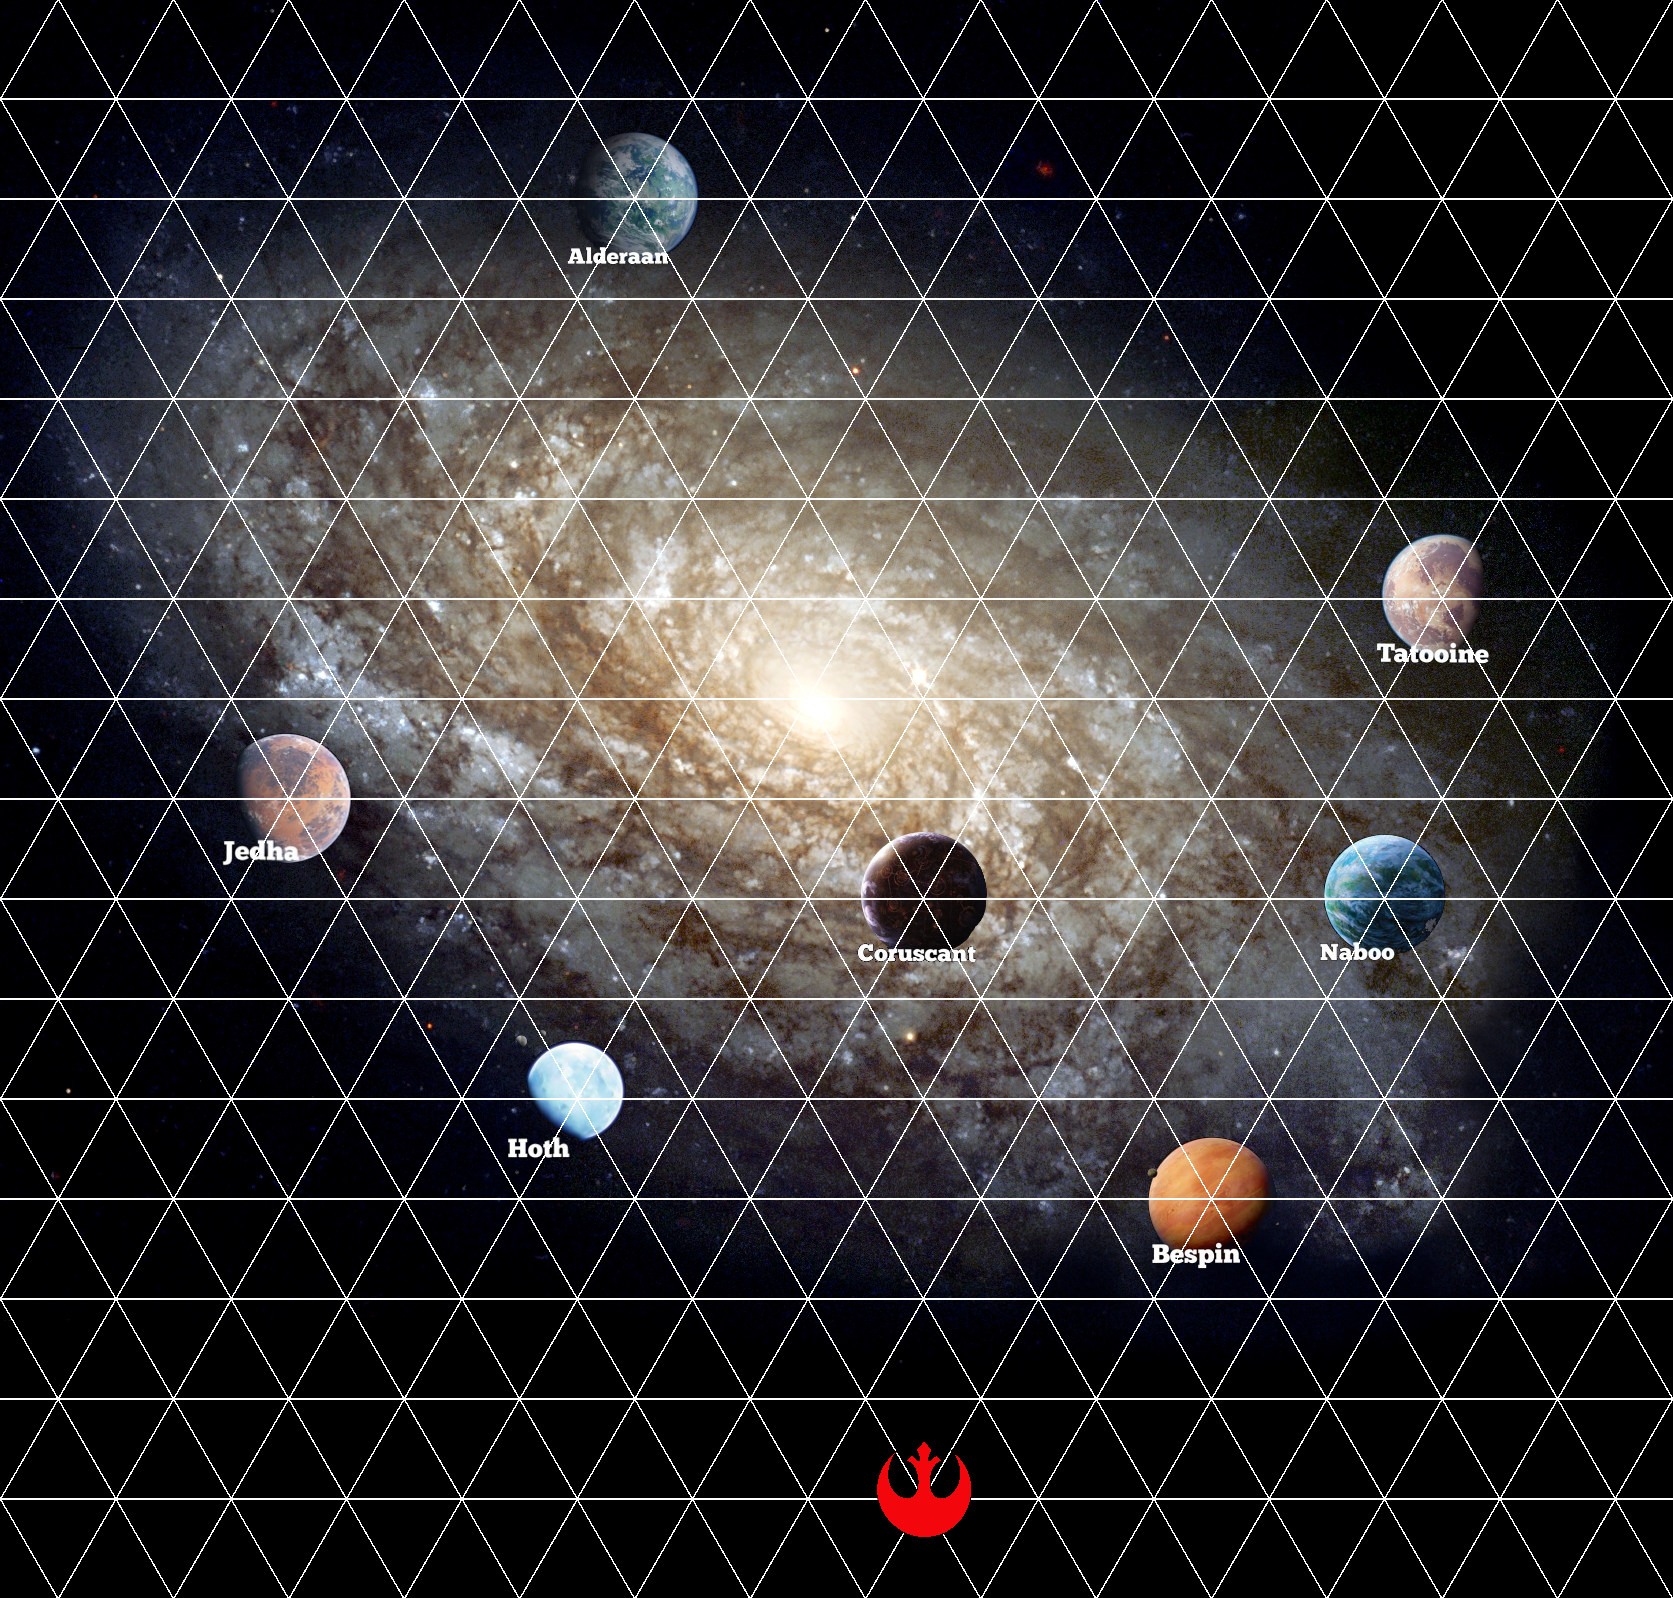
\includegraphics[width=0.8\textwidth]{pic/Map.png}}\end{center}

    {\large \begin{center}{\Large \textbf{Jove \emph{padawan}, la Rebel·lió té una missió per a tu!}}\end{center}

    L'Imperi Galàctic està desenvolupant una nova arma que podria canviar el curs de la guerra. Els nostres espies ens han fet arribar un plànol de l'artefacte, però no han pogut determinar-ne la ubicació. La comandant Organa sospita que es troba amagada prop d'un d'aquests set planetes, però de moment la cerca ha esta infructuosa. El mestre Kenobi ens ha parlat molt bé de tu i volem que facis servir la teva connexió especial amb la \emph{Força} per determinar en quin sistema planetari s'amaga. Per fer-ho cal que segueixis atentament aquestes instruccions:

    \begin{itemize}
        \item Posa el mapa galàctic davant teu i \textbf{situa la teva nau sobre el logotip de l'Aliança Rebel}.
        \item Reparteix les \textbf{set cartes} sobre la taula \textbf{amb les rutes cap amunt}. És molt important que no miris els planetes per no pertorbar la teva intuició.
        \item Una a una, \textbf{selecciona les rutes en l'ordre que et dicti la \emph{Força}} (de vegades tancar els ulls ajuda) i mou la teva nau seguint amb molta cura cadascuna de les rutes.
        \item Quan t'hagis mogut \textbf{sis vegades} i només quedi una carta sobre la taula, atura't! El planeta que estem buscant estarà al dors d'aquesta carta.
        \item Si tens una veritable conexió amb la \emph{Força} t'adonaràs que no et cal girar la carta per saber en quin planeta s'amaga la nova arma de l'Imperi.
    \end{itemize}}

    %%%%%%%%%%%%%%%%%%%%%%%%%%%%%%%%%%%%%%%%%%%%%%%%%%%%%%%%%%%%%%%%%%%%%%%%%%%%

    \newpage
    \thispagestyle{empty}
    \globalcolor{white}  
    \pagecolor{black}
    
    \begin{center}
        {\Large \textbf{Retalla aquestes set cartes, doblega-les per la meitat i enganxa-les amb cola.}}
    \end{center}

    \bigskip\bigskip

    \begin{center}
        \raisebox{4ex}{\rotatebox{90}{\Large\ScissorRightBrokenBottom}}\hspace{-0.5ex}\fcolorbox{white}{black}{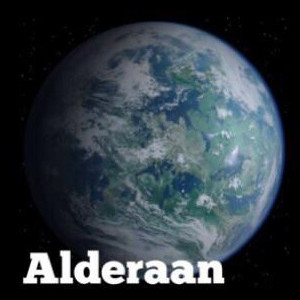
\includegraphics[width=24ex]{pic/A_Planet.jpg}}\fcolorbox{white}{black}{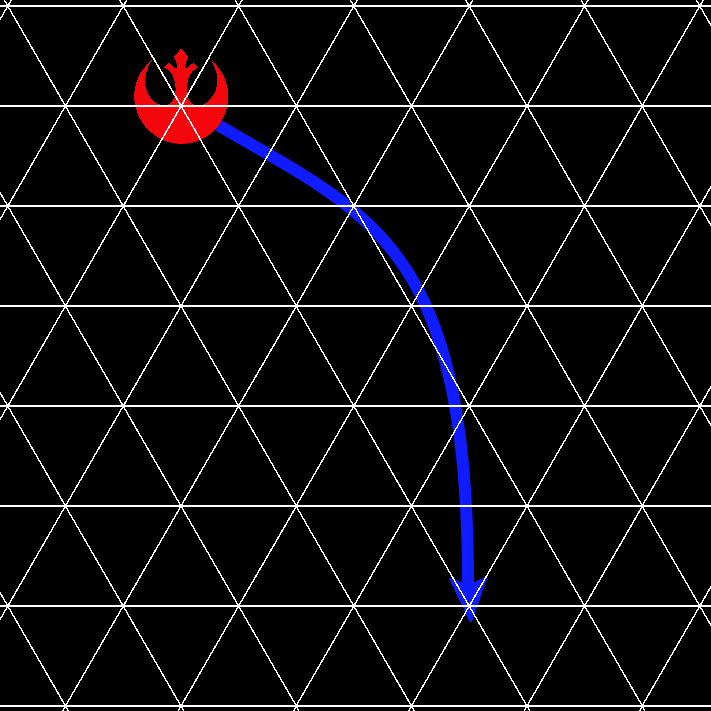
\includegraphics[width=24ex]{pic/A_Clue.png}}\hfill
        \raisebox{4ex}{\rotatebox{90}{\Large\ScissorRightBrokenBottom}}\hspace{-0.5ex}\fcolorbox{white}{black}{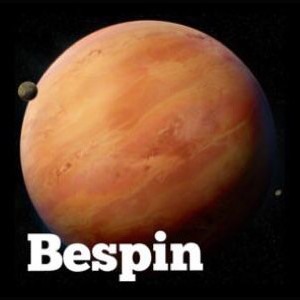
\includegraphics[width=24ex]{pic/B_Planet.jpg}}\fcolorbox{white}{black}{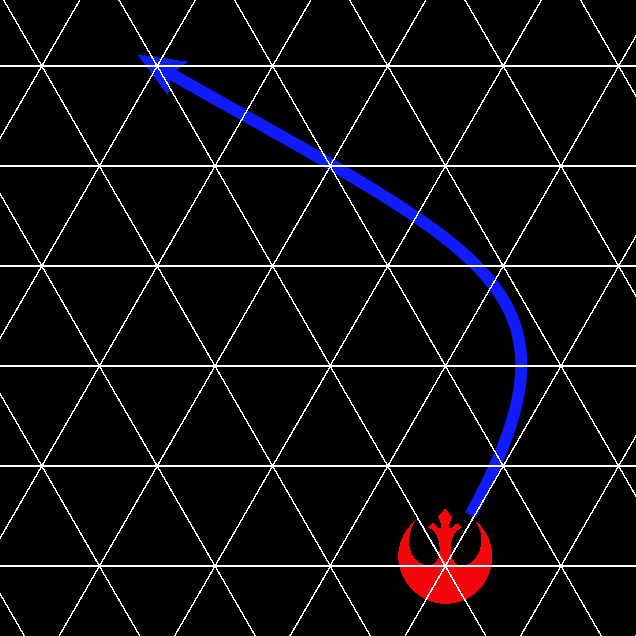
\includegraphics[width=24ex]{pic/B_Clue.png}}\\[5ex]
        \raisebox{4ex}{\rotatebox{90}{\Large\ScissorRightBrokenBottom}}\hspace{-0.5ex}\fcolorbox{white}{black}{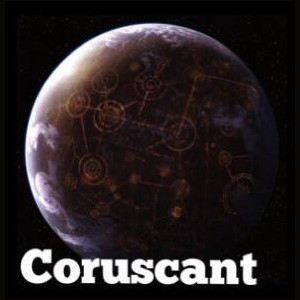
\includegraphics[width=24ex]{pic/C_Planet.jpg}}\fcolorbox{white}{black}{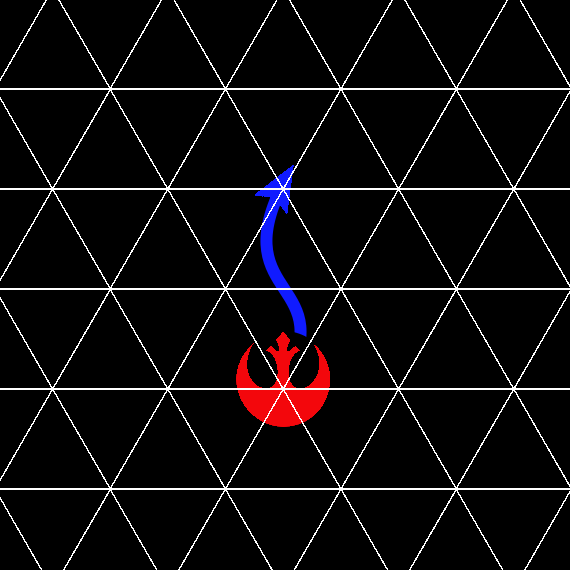
\includegraphics[width=24ex]{pic/C_Clue.png}}\hfill
        \raisebox{4ex}{\rotatebox{90}{\Large\ScissorRightBrokenBottom}}\hspace{-0.5ex}\fcolorbox{white}{black}{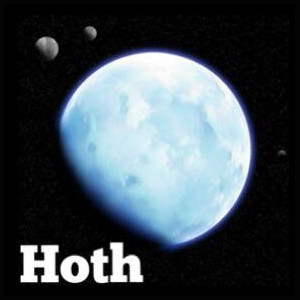
\includegraphics[width=24ex]{pic/H_Planet.jpg}}\fcolorbox{white}{black}{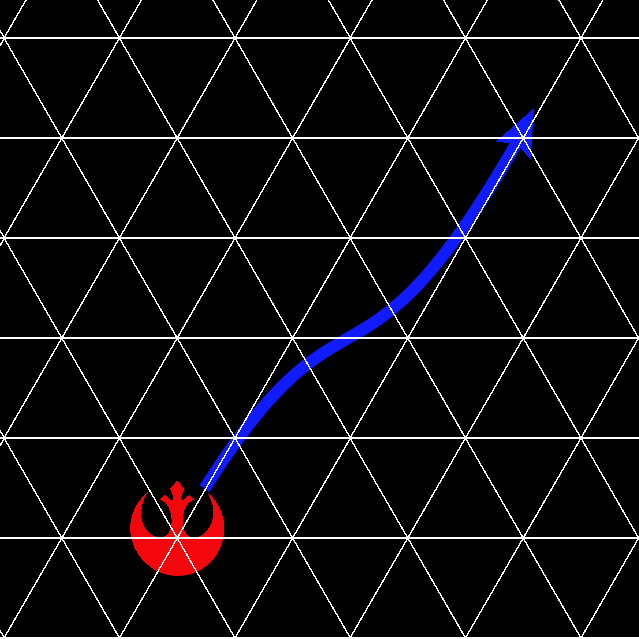
\includegraphics[width=24ex]{pic/H_Clue.png}}\\[5ex]
        \raisebox{4ex}{\rotatebox{90}{\Large\ScissorRightBrokenBottom}}\hspace{-0.5ex}\fcolorbox{white}{black}{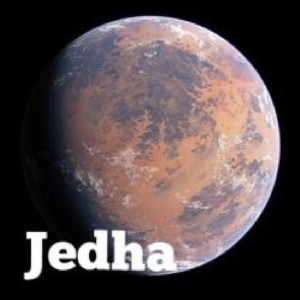
\includegraphics[width=24ex]{pic/J_Planet.jpg}}\fcolorbox{white}{black}{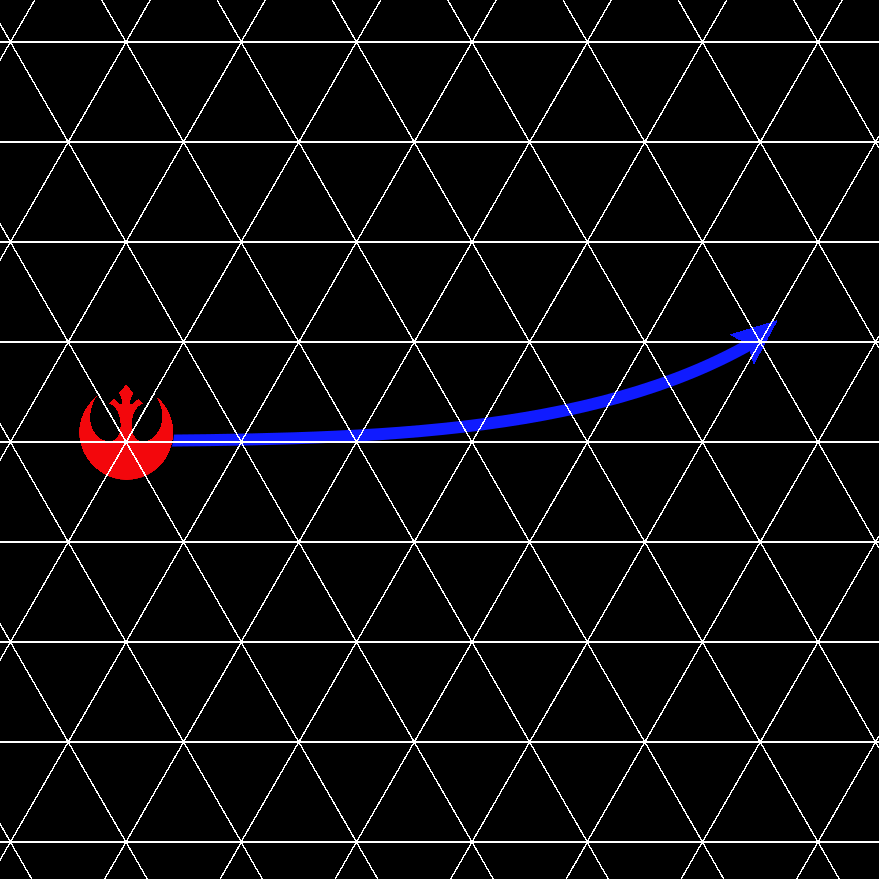
\includegraphics[width=24ex]{pic/J_Clue.png}}\hfill
        \raisebox{4ex}{\rotatebox{90}{\Large\ScissorRightBrokenBottom}}\hspace{-0.5ex}\fcolorbox{white}{black}{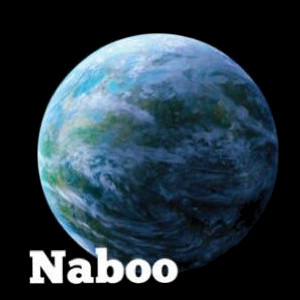
\includegraphics[width=24ex]{pic/N_Planet.jpg}}\fcolorbox{white}{black}{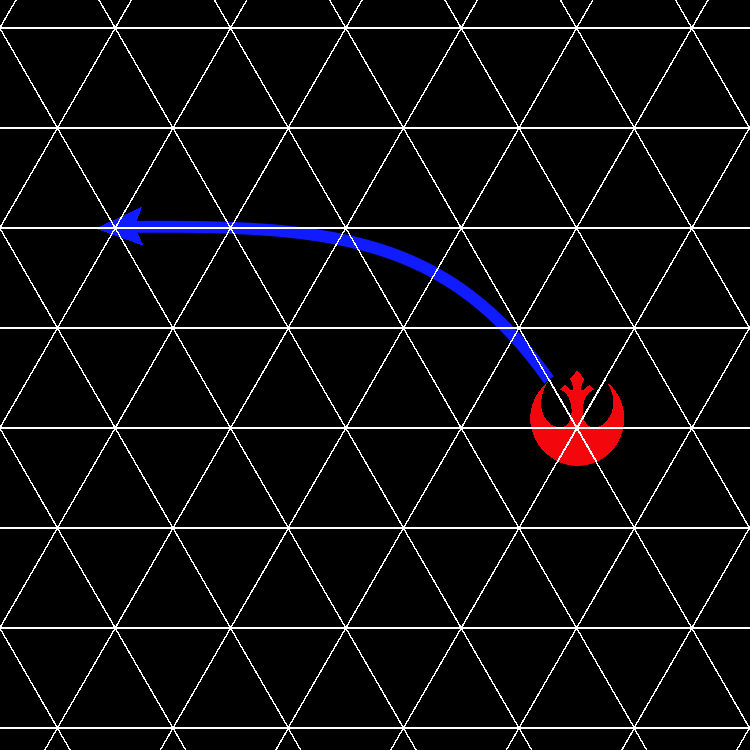
\includegraphics[width=24ex]{pic/N_Clue.png}}\\[5ex]
        \raisebox{4ex}{\rotatebox{90}{\Large\ScissorRightBrokenBottom}}\hspace{-0.5ex}\fcolorbox{white}{black}{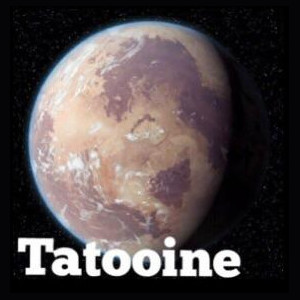
\includegraphics[width=24ex]{pic/T_Planet.jpg}}\fcolorbox{white}{black}{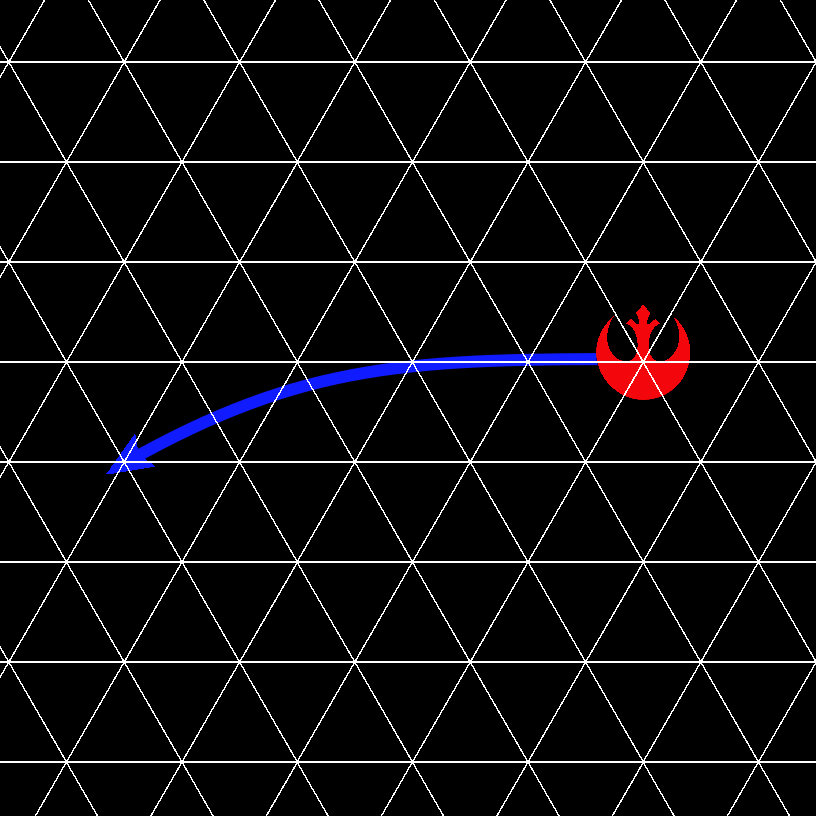
\includegraphics[width=24ex]{pic/T_Clue.png}}
    \end{center}


    %%%%%%%%%%%%%%%%%%%%%%%%%%%%%%%%%%%%%%%%%%%%%%%%%%%%%%%%%%%%%%%%%%%%%%%%%%%%

    \newpage
    \thispagestyle{empty}
    \pagecolor{white}
    \globalcolor{black}
    \begin{center}\vspace{-15ex}
\includegraphics[width=0.5\textwidth]{pic/StarVectors.png}\end{center}

    \begin{center}\frame{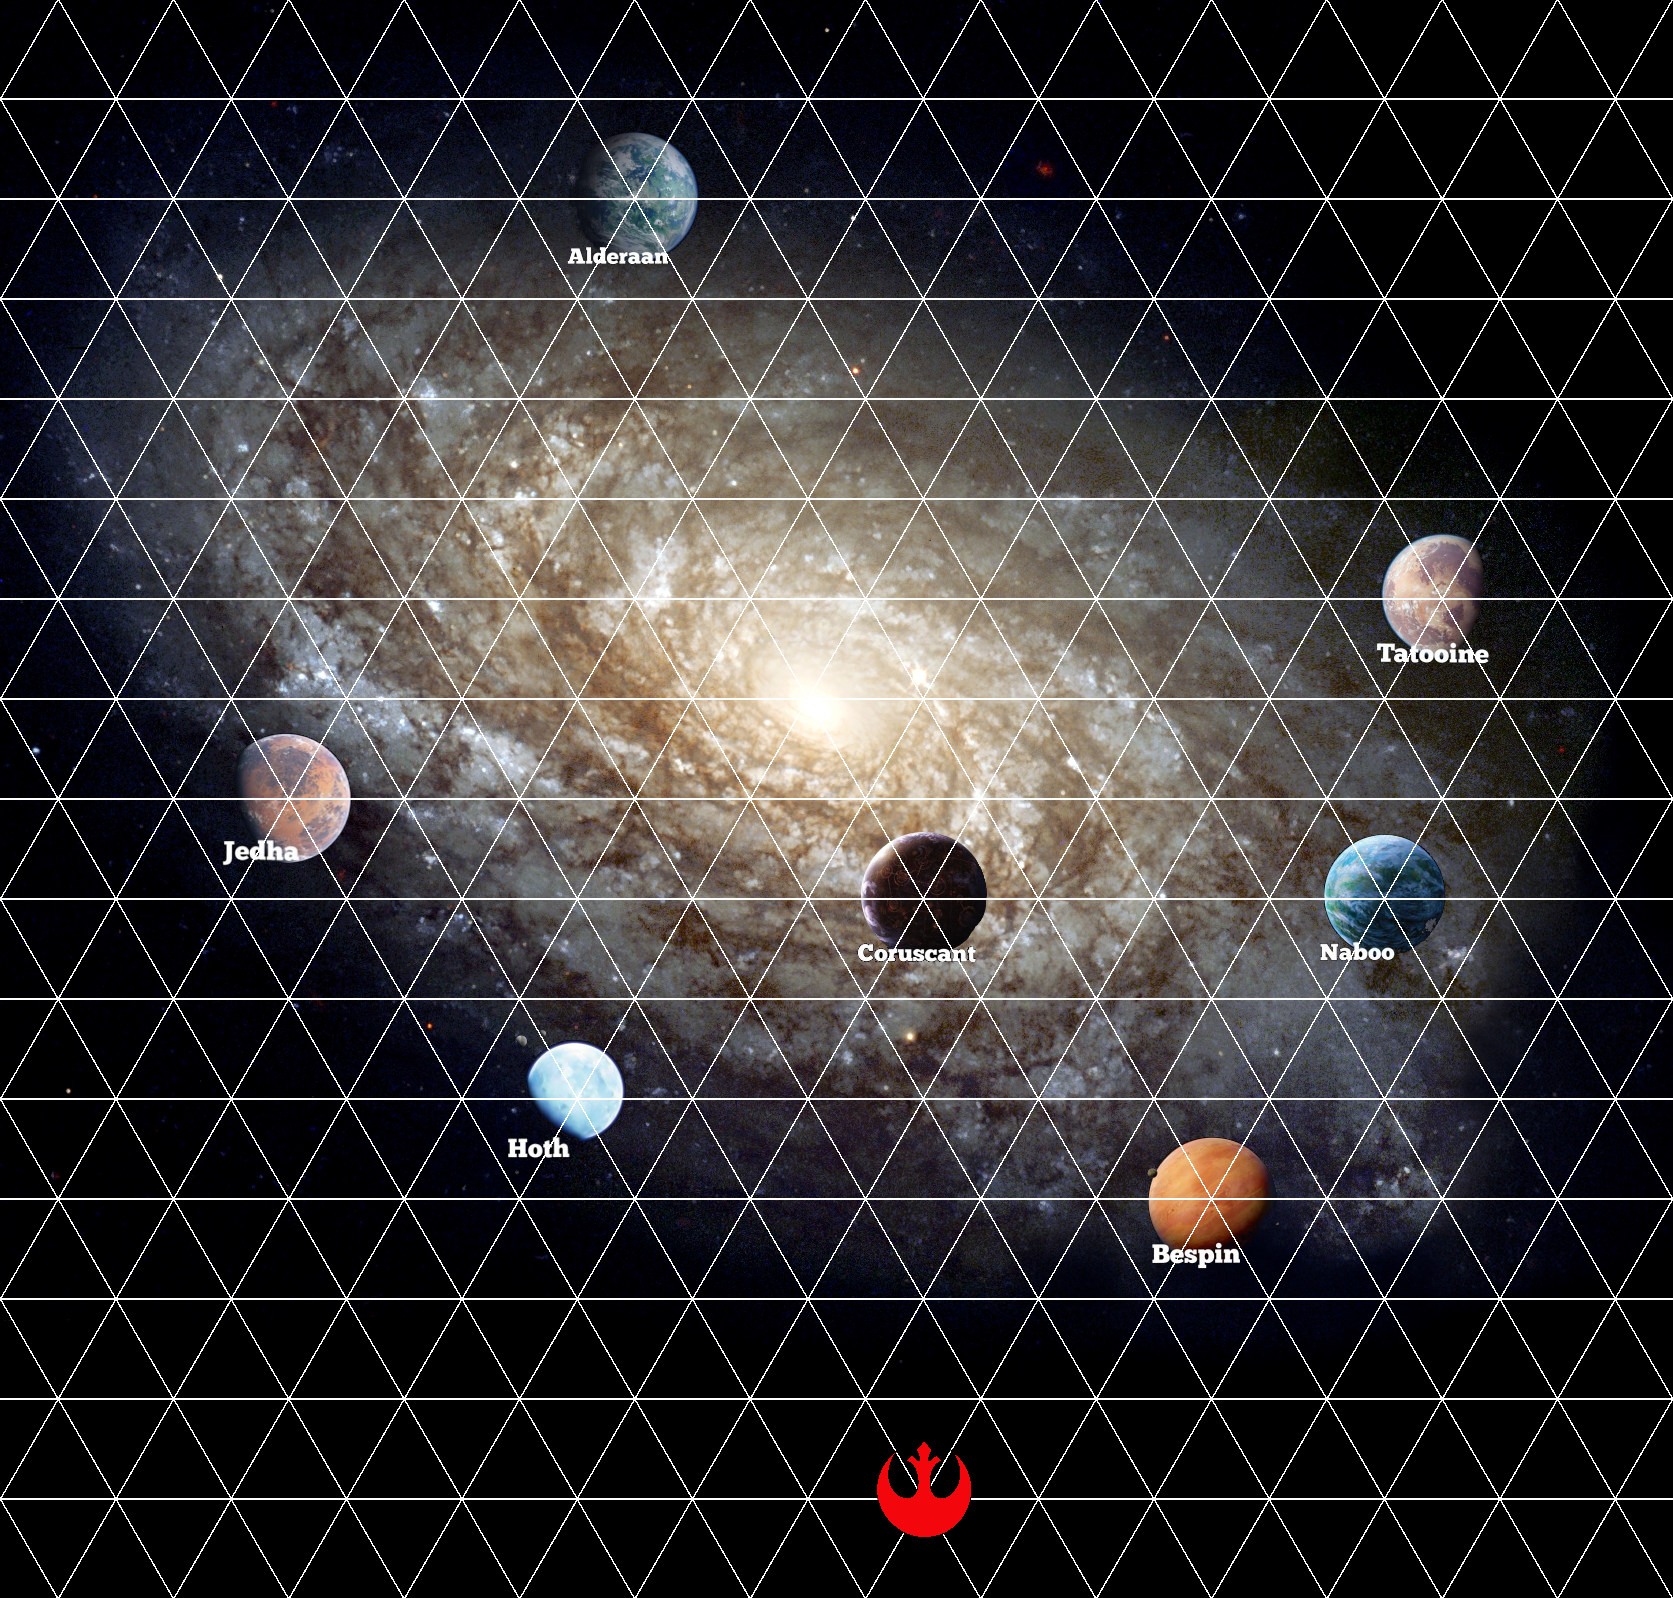
\includegraphics[width=0.8\textwidth]{pic/Map.png}}\end{center}

    {\large \begin{center}{\Large \textbf{Jove \emph{padawan}, la Rebel·lió té una missió per a tu!}}\end{center}

    L'Imperi Galàctic està desenvolupant una nova arma que podria canviar el curs de la guerra. Els nostres espies ens han fet arribar un plànol de l'artefacte, però no han pogut determinar-ne la ubicació. La comandant Organa sospita que es troba amagada prop d'un d'aquests set planetes, però de moment la cerca ha esta infructuosa. El mestre Kenobi ens ha parlat molt bé de tu i volem que facis servir la teva connexió especial amb la \emph{Força} per determinar en quin sistema planetari s'amaga. Per fer-ho cal que segueixis atentament aquestes instruccions:

    \begin{itemize}
        \item Posa el mapa galàctic davant teu i \textbf{situa la teva nau sobre el logotip de l'Aliança Rebel}.
        \item Reparteix les \textbf{set cartes} sobre la taula \textbf{amb les rutes cap amunt}. És molt important que no miris els planetes per no pertorbar la teva intuició.
        \item Una a una, \textbf{selecciona les rutes en l'ordre que et dicti la \emph{Força}} (de vegades tancar els ulls ajuda) i mou la teva nau seguint amb molta cura cadascuna de les rutes.
        \item Quan t'hagis mogut \textbf{sis vegades} i només quedi una carta sobre la taula, atura't! El planeta que estem buscant estarà al dors d'aquesta carta.
        \item Si tens una veritable conexió amb la \emph{Força} t'adonaràs que no et cal girar la carta per saber en quin planeta s'amaga la nova arma de l'Imperi.
    \end{itemize}}

    %%%%%%%%%%%%%%%%%%%%%%%%%%%%%%%%%%%%%%%%%%%%%%%%%%%%%%%%%%%%%%%%%%%%%%%%%%%%
    
    \newpage
    \thispagestyle{empty}

    \begin{center}
        {\Large \textbf{Retalla aquestes set cartes, doblega-les per la meitat i enganxa-les amb cola.}}
    \end{center}

    \bigskip\bigskip

    \begin{center}
        \raisebox{4ex}{\rotatebox{90}{\Large\ScissorRightBrokenBottom}}\hspace{-0.5ex}\fcolorbox{white}{black}{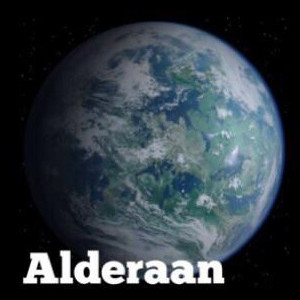
\includegraphics[width=24ex]{pic/A_Planet.jpg}}\fcolorbox{white}{black}{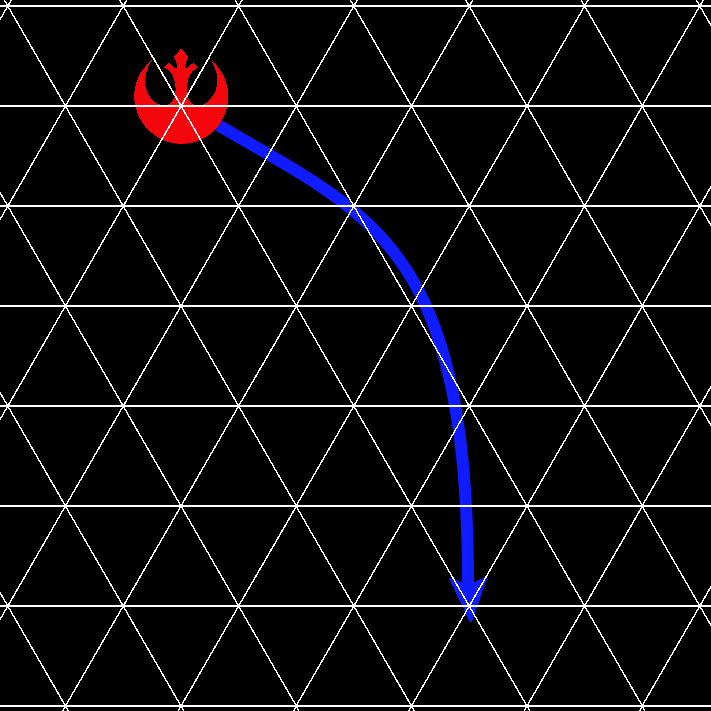
\includegraphics[width=24ex]{pic/A_Clue.png}}\hfill
        \raisebox{4ex}{\rotatebox{90}{\Large\ScissorRightBrokenBottom}}\hspace{-0.5ex}\fcolorbox{white}{black}{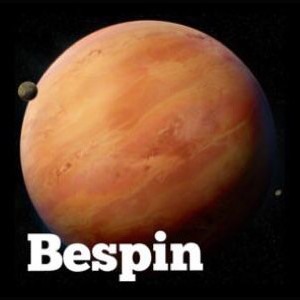
\includegraphics[width=24ex]{pic/B_Planet.jpg}}\fcolorbox{white}{black}{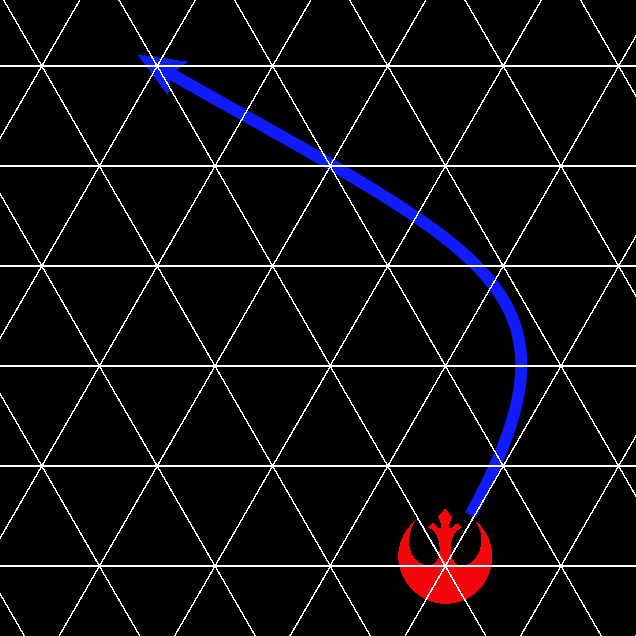
\includegraphics[width=24ex]{pic/B_Clue.png}}\\[5ex]
        \raisebox{4ex}{\rotatebox{90}{\Large\ScissorRightBrokenBottom}}\hspace{-0.5ex}\fcolorbox{white}{black}{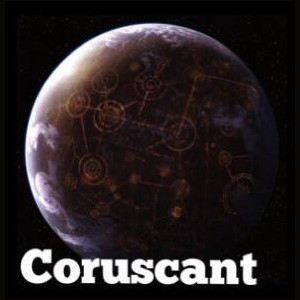
\includegraphics[width=24ex]{pic/C_Planet.jpg}}\fcolorbox{white}{black}{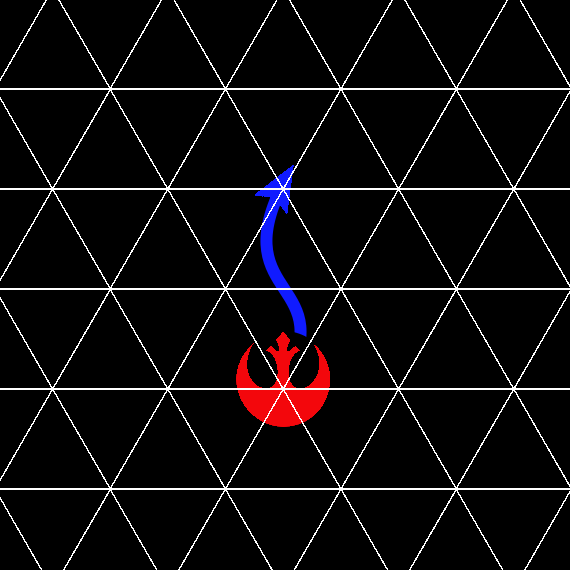
\includegraphics[width=24ex]{pic/C_Clue.png}}\hfill
        \raisebox{4ex}{\rotatebox{90}{\Large\ScissorRightBrokenBottom}}\hspace{-0.5ex}\fcolorbox{white}{black}{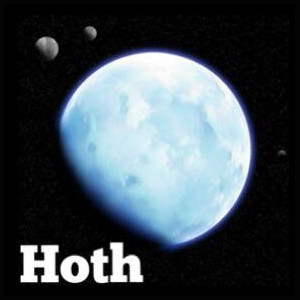
\includegraphics[width=24ex]{pic/H_Planet.jpg}}\fcolorbox{white}{black}{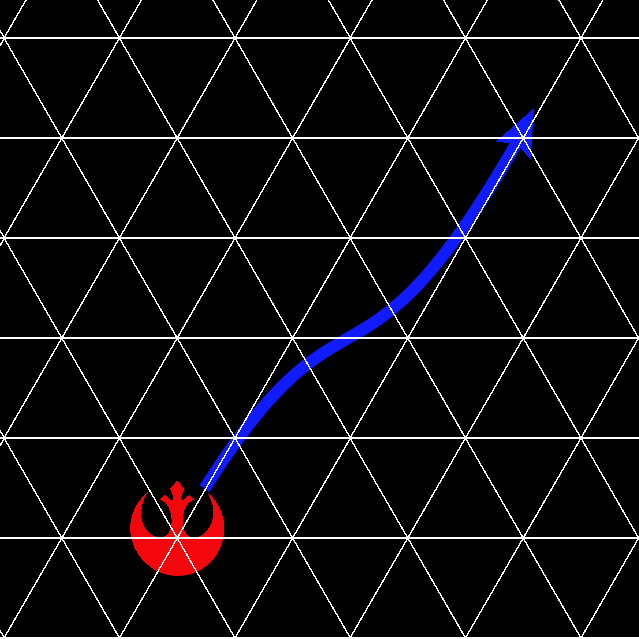
\includegraphics[width=24ex]{pic/H_Clue.png}}\\[5ex]
        \raisebox{4ex}{\rotatebox{90}{\Large\ScissorRightBrokenBottom}}\hspace{-0.5ex}\fcolorbox{white}{black}{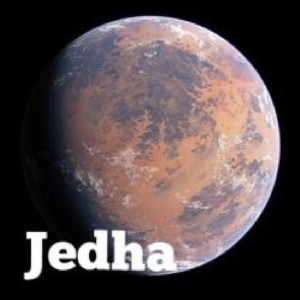
\includegraphics[width=24ex]{pic/J_Planet.jpg}}\fcolorbox{white}{black}{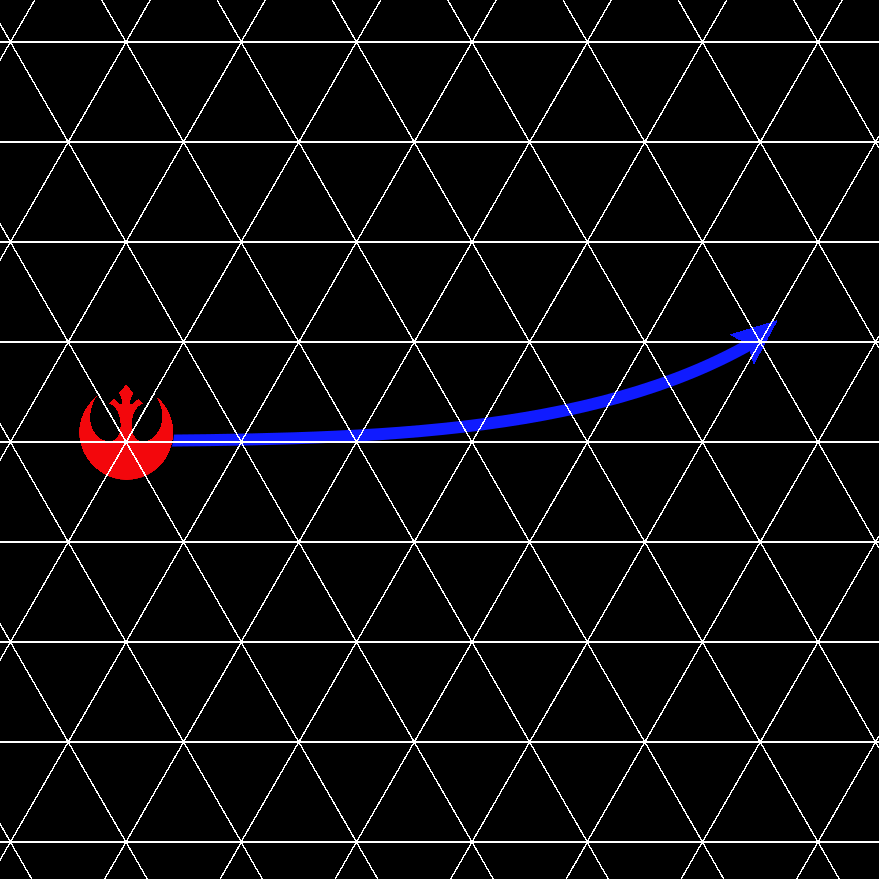
\includegraphics[width=24ex]{pic/J_Clue.png}}\hfill
        \raisebox{4ex}{\rotatebox{90}{\Large\ScissorRightBrokenBottom}}\hspace{-0.5ex}\fcolorbox{white}{black}{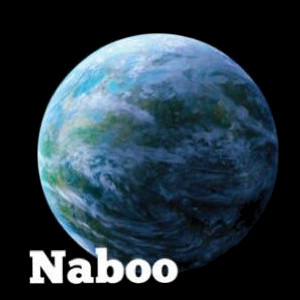
\includegraphics[width=24ex]{pic/N_Planet.jpg}}\fcolorbox{white}{black}{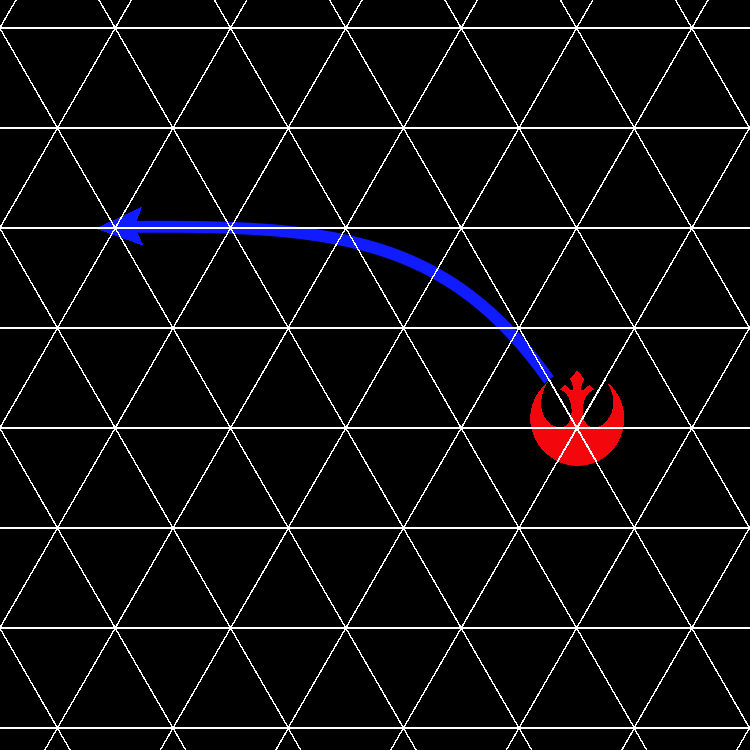
\includegraphics[width=24ex]{pic/N_Clue.png}}\\[5ex]
        \raisebox{4ex}{\rotatebox{90}{\Large\ScissorRightBrokenBottom}}\hspace{-0.5ex}\fcolorbox{white}{black}{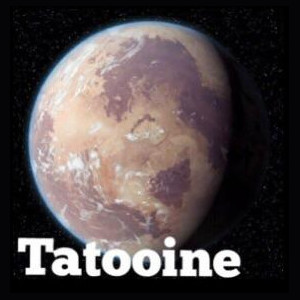
\includegraphics[width=24ex]{pic/T_Planet.jpg}}\fcolorbox{white}{black}{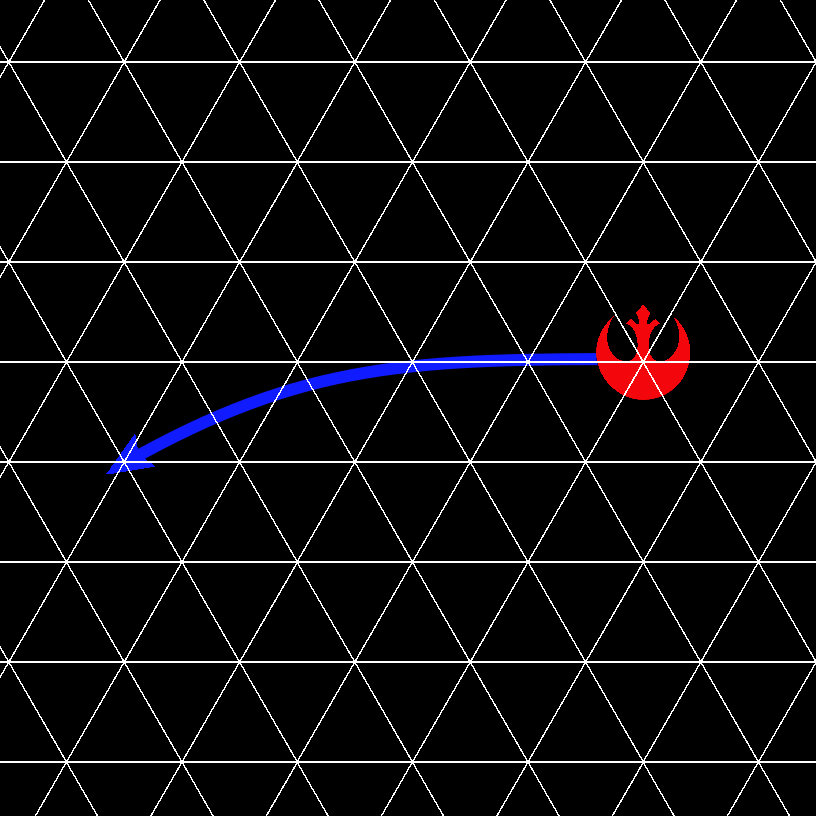
\includegraphics[width=24ex]{pic/T_Clue.png}}
    \end{center}
    
    
\end{document}
